\documentclass[11pt]{article}
% Basic Packages for Encoding (Input AND Output) and Langauge Support
\usepackage[utf8]{inputenc}
\usepackage[T1]{fontenc}
\usepackage[french]{babel}

% Change Layout with a User-Friendly Interface
\usepackage[margin=1in]{geometry}

% Include Pictures with a User-Friendly Interface
\usepackage{graphicx}
\usepackage{float}

% Extended Math Support from the Famous 'American Mathematical Society'
\usepackage{amsmath}
\usepackage{amsfonts}
\usepackage{amssymb}

% Just for Demonstration Purposes
\usepackage[math]{blindtext}

% For use on computer
\usepackage{hyperref}

% For table color
\usepackage{xcolor,colortbl}

% Titre
\usepackage[affil-it]{authblk}
\title{\textbf{TP Pendule Balistique}}
\author{Camille Yerly, Romain Blondel}
\affil{2M8, Gymnase Auguste Piccard}
\date{10 octobre 2022}

\begin{document}

\maketitle

\section{But}
Le but de ce travail pratique est d'évaluer un instrument de mesure, le pendule balistique, permettant de déterminer la vitesse d'un projectile à la sortie d'un canon sans avoir à parcourir la distance correspondant à la portée du canon qui pourrait être de plusieurs centaines de mètres. Nous comparons donc une mesure directe de la portée à la méthode du pendule balistique.

\section{Introduction théorique}
L'armée est un mécène important de la recherche scientifique. Il est donc presque inévitable de finir par travailler sur des sujets qui y sont lié, comme la mesure de la vitesse d'un projectile depuis un canon. C'est utile par exemple pour pouvoir prédire où il va atterrir selon d'autres paramètres extérieurs. De plus c'est un sujet intéressant du point de vue théorique pour appliquer différents modèles physique, et réfléchir depuis ces expérience à petite échelle à la pertinence et l'utilité des unes par rapport aux autres selon la vitesse à mesuré. On s'attend à constater un avantage à utiliser le pendule balistique par sa praticité du au fait qu'il peut être plus compacte que des tirs complets, mais on pourrait en découvrir d'autres au fil de l'expérience, ou des désavantages par rapport à la balistique classique selon le cas.
\\
Afin de réaliser les calculs, nous avons utilisé plusieurs notions théoriques présentées ci-dessous.
\subsection{Expérience 1 - Balistique} \label{subsec:intro1}
La bille se trouve dans un MRUA. Nous pouvons donc poser l'équation horaire du mouvement :
$$ \vec{r}(t)=\dfrac{1}{2} \cdot \vec{a} \cdot t^2+\vec{v}_0 \cdot t + \vec{r}_0$$
 Avec :
\begin{itemize}
 \item $t$ : le temps $[s]$
 \item $\vec{r}(t)$ : le vecteur position selon le temps $[m]$
 \item $\vec{a}$ : le vecteur accélération $[m/s^2]$ 
 \item $\vec{v}_0$ : le vecteur vitesse initiale de la bille $[m/s]$  
 \item $\vec{r}_0$ : le vecteur position initiale $[m]$
\end{itemize}
Et lorsque nous travaillons en composantes : $$\begin{pmatrix} x(t)\\y(t) \end{pmatrix}=\dfrac{1}{2} \cdot \begin{pmatrix} 0\\g \end{pmatrix} \cdot t^2 +\begin{pmatrix} v_0\\0 \end{pmatrix} \cdot t+0$$
Ce qui nous permet de poser : \begin{center} 
$x(t)=v_0 \cdot t$ \\
$y(t)= \dfrac{1}{2} \cdot g \cdot t^2$
\end{center}
La première relation lie l'inconnue recherchée, la vitesse $v_0$, à la distance mesurée. Cependant la durée de chute $t_c$ est encore inconnue. \\La deuxième relation lie
la hauteur du canon $h$ au temps de chute $t_c$, la gravité terrestre $g$ étant connue. \begin{center}
$d=v_0 \cdot t_c$\\
$h= \dfrac{1}{2} \cdot g \cdot t^2_c$
\end{center}
\subsection{Expérience 2 - Pendule} \label{subsec:intro2}
La bille sort du canon et s'incruste dans le pendule. Lors de cet événement la quantité de mouvement reste constante : \begin{center}
$\sum\limits_{i}\vec{p}_i=constante$\\
$m_b \cdot v_0=(m_b+m_p) \cdot v_p$
\end{center} Avec:
\begin{itemize}
 \item $m_b$ : la masse de la bille $[Kg]$
 \item $v_0$ : la vitesse initiale de la bille $[m/s]$
 \item $m_p$ : la masse du pendule $[Kg]$
 \item $v_p$ : la vitesse du pendule au moment de l'impact avec la bille $[m/s]$
\end{itemize}
Puis, lorsque le pendule est en mouvement, la loi de conservation de l'énergie mécanique s'applique.$$E_{mec}=E_{pot}+E_{cin}=constante$$ Initialement, la totalité de l'énergie $E_{mec1}$ est cinétique et on peut considérer l'énergie potentielle nulle. A l'apogée, lorsque le pendule s'arrête $E_{mec2}$, l'énergie cinétique est nulle et s'est intégralement convertie en énergie potentielle. \begin{center}
$E_{mec1}=E_{mec2}$\\
$\dfrac{1}{2} \cdot (m_b+m_p) \cdot v_p^2=(m_b+m_p)\cdot g \cdot \Delta h$
\end{center} Ce qui se simplifie : $$\dfrac{1}{2} \cdot v_p^2=g \cdot \Delta h$$ Avec : 
\begin{itemize}
 \item $\Delta h$ : l'élévation maximale du pendule.\\ L'angle $\alpha$ mesuré lors de l'expérience permet le calcul de $\Delta h$ 
\end{itemize}

\section{Principe de mesure et description}
Dans la première expérience, nous allons mesuré la distance d'impact d'un tir de canon pour en calculer la vitesse initiale via la balistique (voir Section \ref{subsec:intro1}). \\
Dans la seconde, nous allons faire de même, en passant par la conservation de la quantité de mouvement et de l'énergie mécanique, en mesurant l'angle d'un "pendule balistique" (voir Section \ref{subsec:intro2}).
\subsection{Matériel}
\paragraph*{} Afin de réaliser la première expérience nous avons utilisé :
\begin{itemize}
\item Papier carbone
\item Bille en métal
\item Canon  
\item Mètre
\item Balance
\end{itemize}
\paragraph*{} Pour la deuxième expérience, nous avons utilisé :
\begin{itemize}
\item Pendule balistique (pouvant être lesté)
\item Bille en métal
\item Canon  
\item Mètre
\item Balance
\item Rapporteur
\end{itemize}

\subsection{Déroulement}
\paragraph*{} Pour la première expérience :
\begin{enumerate}
\item Nous avons mesuré la hauteur de départ de la bille dans le canon.
\item Nous avons placé la feuille de papier carbone sur une feuille blanche afin de reporter les points d'atterrissage de la bille pour chaque tir.
\item Nous avons effectué six tirs pour chacun des trois crans du canon, variant ainsi la vitesse initiale de la bille. Nous avons mesuré les distances d'atterrissage pour chaque tir. 
\end{enumerate}
\paragraph*{} Pour la deuxième expérience:
\begin{enumerate}
\item Nous avons mesuré la masse de la bille, la masse du pendule balistique lesté avec la bille à l'intérieur, ainsi que la longueur du centre de masse jusqu'à l'axe de rotation du pendule.
\item Nous avons effectué trois tir pour chaque cran du canon en rapportant l'angle maximal atteint par le pendule à chaque reprise. 
\item Nous avons enlevé le lest du pendule et avons reproduit les étapes 1 et 2.
\end{enumerate}

\subsection{Schémas}
\begin{figure}[H]
\center
\label{figure:schem-exp1}
\includegraphics[scale=0.7]{Schéma/exp1-schem.pdf}
\caption{Schéma de l'expérience 1}
\end{figure}

\begin{figure}[H]
\center
\label{figure:schem-exp2}
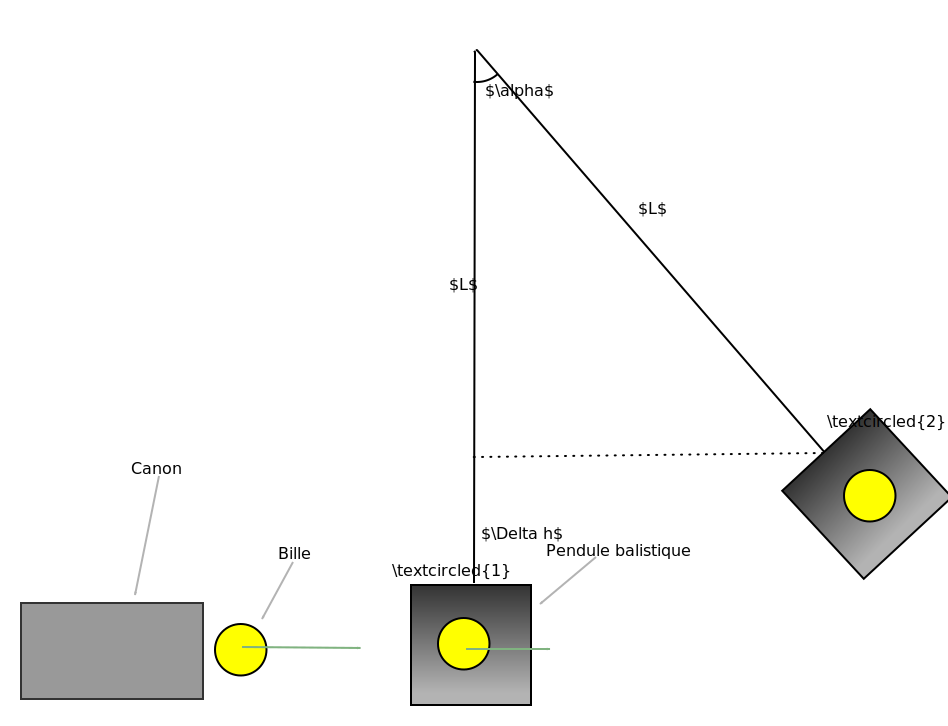
\includegraphics[scale=0.7]{Schéma/exp2-schem.pdf}
\caption{Schéma de l'expérience 2}
\end{figure}

\section{Résultats et calculs}
\subsection{Expérience 1}
Pour cette première expérience, nous avons mesuré la hauteur de départ du projectile, $h = 6.3 \ [cm]$, ainsi que la distance entre le canon et l'impacte (seul la moyenne sur 6 valeurs est consignée - voir Table \ref{table:dist_e1}).

\begin{table}[H]
\center
\begin{tabular}{|>{\columncolor{gray}}c||c|>{\columncolor{lightgray}}c|c|}
\hline
\rowcolor{gray} Cran & 1 & 2 & 3 \\ \hline
$d_{moy} \ [cm]$ & 25.1 & 41.4 & 56.4\\ \hline
\end{tabular}
\caption{Distance d’impacte}
\label{table:dist_e1}
\end{table}

Puis de $h$ via les formules de balistiques, et connaissant l'accélération terrestre $g=9.81 \ \left[ \frac{m}{s^2} \right]$, on peut calculer le temps de chute $h = \frac{1}{2} \cdot g \cdot t^2 \Leftrightarrow t = \sqrt{\frac{2h}{g}} \approx 0.113 \ [s]$. De là on peut calculer la vitesse via $v = \frac{d}{t}$ (voir Table \ref{table:dist_e2}).

\begin{table}[H]
\center
\begin{tabular}{|>{\columncolor{gray}}c||c|>{\columncolor{lightgray}}c|c|}
\hline
\rowcolor{gray} Cran & 1 & 2 & 3 \\ \hline
$v \ \left[ \frac{m}{s} \right]$ & 2.21 & 3.65 & 4.98\\ \hline
\end{tabular}
\caption{Vitesse de propulsion}
\label{table:dist_e2}
\end{table}

\subsection{Expérience 2}
Cette partie c'est faite en deux fois : l'une avec le pendule balistique sans leste, et une avec. Dans les deux cas les paramètres mesurés sont les mêmes. Tout d'abord la masse de la bille $m = 66 \ [g]$, et la masse totale du pendule balistique et de la bille $M_{totale} = 206.6 \ [g]$ et $M_{totale \ leste} = 305.8 \ [g]$, ainsi que les bras de levier $L = 26.4 \ [cm]$ et $L_{leste} = 28.3 \ [cm]$. Nous avons dès lors pris la mesure des angles maximaux du pendule pour chaque cran (la moyenne de 3 tirs, à part sur les crans 2 et 3 sans leste où ce fut sur 4 - voir Table \ref{table:angles_e2}).

\begin{table}[H]
\center
\begin{tabular}{|>{\columncolor{gray}}c||c|>{\columncolor{lightgray}}c|c|>{\columncolor{lightgray}}c|c|>{\columncolor{lightgray}}c|}
\hline
\rowcolor{gray} Cran & \multicolumn{2}{c|}{1} & \multicolumn{2}{c|}{2} & \multicolumn{2}{c|}{3} \\ \hline
$\alpha \ [^\circ]$ & 28.5 & 16.833 & 44.625 & 26.833 & 63.875 & 37.333 \\ \hline
\end{tabular}
\caption{Angles du pendule balistique (les mesures grisées sont avec leste, les autres sans)}
\label{table:angles_e2}
\end{table}

De ces mesures on peut calculer la différence de hauteur entre la position de départ du pendule et celle maximale par une relation trigonométrique (voir Figure \ref{figure:schem-exp2}) $\Delta h = L - L \cdot \cos \alpha = L(1-\cos \alpha)$. De là, via la conservation de l'énergie mécanique : 
$$E_{mec1} = E_{mec2} \Leftrightarrow \frac{1}{2} \cdot M \cdot v_{1}^2 + M \cdot g \cdot h_{1} = \frac{1}{2} \cdot M \cdot v_{2}^2 + M \cdot g \cdot h_{2} \Leftrightarrow $$
$$ \frac{1}{2} \cdot v_{1}^2 + g \cdot h_{1} = g \cdot h_{2} \Leftrightarrow \frac{1}{2} v_{1}^2 = g(h_{2}-h_{1}) = g \cdot \Delta h \Leftrightarrow v_{1}^2 = 2 \cdot g \cdot \Delta h \Leftrightarrow v_{1} = \sqrt{2 \cdot g \cdot \Delta h}$$

Alors on peut obtenir la vitesse initiale via la conservation de la quantité de mouvement :
$$\sum_{i} \vec{p_{i}} = constante \Leftrightarrow m \cdot v_{0} = M_{totale} \cdot v_{1} \Leftrightarrow v_{0} = \frac{M_{totale} \cdot v_{1}}{m}$$

On peut donc résumer numériquement ces résultats selon nos mesures (cf. Table \ref{table:calculs_e2}).

\begin{table}[H]
\center
\begin{tabular}{|>{\columncolor{gray}}c||c|>{\columncolor{lightgray}}c|c|>{\columncolor{lightgray}}c|c|>{\columncolor{lightgray}}c|}
\hline
\rowcolor{gray} Cran & \multicolumn{2}{c|}{1} & \multicolumn{2}{c|}{2} & \multicolumn{2}{c|}{3} \\ \hline
$\Delta h \ [m]$ & 0.032 & 0.012 & 0.076 & 0.030 & 0.148 & 0.058 \\ \hline
$v_{1} \ \left[ \frac{m}{s} \right]$ & 0.792 & 0.488 & 1.222 & 0.773 & 1.703 & 1.067 \\ \hline
$v_{0} \ \left[ \frac{m}{s} \right]$ & 2.480 & 2.260 & 3.825 & 3.583 & 5.330 & 4.942 \\ \hline
\end{tabular}
\caption{Calculs de la vitesse initiale (les mesures grisées sont avec leste, les autres sans)}
\label{table:calculs_e2}
\end{table}

\subsection{Erreur}
On remarque assez vite des résultats différents pour la vitesse initiale entre les deux expérience, ainsi que au sein même de la seconde expérience. Il est donc intéressant de calculer l'erreur entre ceux-ci, ainsi que entre les expérience en globale (moyenne sur le pendule comparé a la balistique - voir Table \ref{table:err}).

\begin{table}[H]
\center
\begin{tabular}{|>{\columncolor{gray}}c|c|>{\columncolor{lightgray}}c|c|>{\columncolor{lightgray}}c|}
\hline
\rowcolor{gray} \cellcolor{black} & $\Delta(v_{exp1}, v_{exp2}) \%$ & $\Delta(v_{exp1}, v_{exp2 \ leste}) \%$ & $\Delta(v_{exp2}, v_{exp2 \ leste}) \%$ & $\Delta(v_{exp1}, v_{exp2 \ moy}) \%$ \\ \hline
$v_{cran \ 1}$ & 10.70 & 2.00 & 8.87 & 6.55 \\ \hline
$v_{cran \ 2}$ & 4.50 & 1.97 & 6.34 & 1.37 \\ \hline
$v_{cran \ 3}$ & 6.63 & 0.70 & 7.28 & 3.10 \\ \hline
\end{tabular}
\caption{Erreur entre les mesures}
\label{table:err}
\end{table}

\subsection{Incertitudes} \label{subsec:incert}
Dans l'expérience 1, la mesure de la distance a un étalement de l'ordre de 2.0 $[cm]$, donc une incertitude 1$\sigma$ de l'ordre de 0.7$[cm]$.
Par rapport a une distance de 25 a 56 $[cm]$, cela représente 2.8 a 1.2\% d'incertitude sur la mesure.
L'évaluation du temps de vol est plus précis (0.5 $[mm]$ / 63 $[mm]$ = 0.7\%) et pourrait facilement être amélioré en augmentant la hauteur du canon.
Au final l'incertitude intrinsèque de $v_0$ dans l'expérience 1 est entre 3.5\% et 2.0\%.\\
Dans l'expérience 2, la mesure de l'angle a un étalement de 1[°] pour des valeurs de 16 a 63[°], ce qui implique des incertitude de 7\% (respectivement 2\%) pour un angle mesure de 6[°] (respectivement 63 [°]).
Il est donc évidant qu'il faut optimiser le pendule pour que l'angle mesure soit relativement haut.

\subsection{Compléments} \label{subsec:comp}
Comme vu dans la Table \ref{table:err} précédente, l'erreur varie beaucoup. De fait on peut s'interroger sur la sensibilité de la mesure sur la vitesse initiale calculée. De fait on peut essayer de voir la vitesse selon l'angle mesuré dans l'expérience 2 en faisant varier les conditions initiales. Pour ce faire on va reprendre la formule $v_{0} = \frac{M_{totale} \cdot v_{1}}{m} = \frac{M_{totale} \cdot \sqrt{2 \cdot g \cdot \Delta h}}{m} =  \frac{M_{totale} \cdot \sqrt{2 \cdot g \cdot L(1-\cos \alpha)}}{m}$ (voir Figure \ref{figure:graph_vit_angle}).

\begin{figure}[H]
\center
\includegraphics[scale=1]{Graph/vit_angle_plt.pdf}
\caption{Vitesse initiale selon l'angle dans l'expérience 2 ($m_{bille} = 0.05 \ [Kg]$)}
\label{figure:graph_vit_angle}
\end{figure}

De plus on peut estimer l'énergie perdue lors de l'expérience 1. Considérons une approximation comme quoi la vitesse est constante comme celle de départ (approximation basse) et que la distance de vol correspond à la distance horizontal et vertical (approximation haute). En estimant le rayon de la bille à $r = 1 \ [cm]$, le coefficient de traînée de la sphère à $C_x = 0.47$ et la densité de l'air à $\rho = 1.292 \ [Kg/m^3]$, et la surface de la sphère étant $S = 4 \cdot \pi \cdot r^2$, alors avec la formule suivante pour les frottements de l'air $F_f = \frac{1}{2} \cdot \rho \cdot S \cdot C_x \cdot v^2$ alors l'énergie perdue en frottement est de $\Delta E = F_f \cot d_{vol} = F_f \cdot (h + d)$. De fait on peut comparer la proportion d'énergie perdue avec celle de l'énergie cinétique donnée au départ $E_{cin} = \frac{1}{2} \cdot m \cdot v^2$ donc $E_{frott} / E_{cin} = \frac{\rho \cdot S \cdot C_x \cdot (h+d)}{m}$ car les vitesses et facteurs $\frac{1}{2}$ se simplifient (voir Table \ref{table:frott}).

\begin{table}[H]
\center
\begin{tabular}{|>{\columncolor{gray}}c||c|>{\columncolor{lightgray}}c|c|}
\hline
Cran & 1 & 2 & 3 \\ \hline
$E_{frott} / E_{cin} \ [\%]$ & 0.36 & 0.55 & 0.72 \\ \hline
\end{tabular}
\caption{Énergie perdue par frottement de l'air}
\label{table:frott}
\end{table}

\section{Discussion des résultats}
Les résultats paraissent assez cohérents malgré des taux d'erreurs assez variables. Dans la première expérience, nous avons une vitesse évoluant linéairement avec la distance mesurée, sujette à une faible erreur car les impacts était globalement peu éparpillés, car la hauteur de chute et donc le temps de chute sont estimés constant dans ce modèle. Néanmoins cette approximation fonctionne sur des échelles relativement petite, car la quantité d'énergie perdue en frottements de l'air dépend principalement de la distance de vol multipliée par un facteur constant (cf. Section \ref{subsec:comp}). Dans notre cas, c'est moins de $1 \ \%$ de l'énergie que l'on donne au système (voir Table \ref{table:frott}). De fait nous pouvons considérer ces résultats comme fiables. \\
Dans la seconde expérience, on s'appuie sur un modèle plus complexe, le pendule balistique et la conservation de l'énergie, afin d'avoir une méthode applicable à des échelle plus grandes.En effet, via la Figure \ref{figure:graph_vit_angle}, nous observons que l'on peut mesurer des vitesses plus grande en augmentant le bras de levier, ainsi qu'un panel plus large en augmentant le leste sur le pendule. De plus on remarque une croissance moindre en 0 et 30 [°], ce qui indique une plus grande sensibilité à la casse et qui est aussi visible dans l'incertitude sur la mesure (voir Section \ref{subsec:incert}). Finalement, il est important de noter que avec moins de leste, impliquant une moins grande inertie, le système est plus sensible, et donne des résultats moins précis, comme en témoigne la nécessité de faire plus de mesure (pour la Table \ref{table:angles_e2}).\\
Ces points se voient aussi dans l'erreur, où la vitesse au cran 1 est celle avec le plus d'erreur et est globalement considérée comme de précision faible à acceptable, là ou les crans 2 et 3 sont globalement de bonne précision. De plus on voit que le pendule lesté est celui le plus proche du tir balistique, avec un précision globalement excellente. Ce résultats est aussi prévisible à l'aide du graphe évoqué précédemment, dans lequel on voit que un pendule bien lesté est idéal.\\
Finalement, si l'on souhaitait appliquer ça à plus grande échelle, le pendule est plus pratique qu'un tir balistique est sera aussi plus précis à un certain point, mais il nécessite une certaine calibration. 

\section{Conclusion}
En conclusion, les mesures de vitesse à la sortie du canon sont assez satisfaisante. En effet, elles permettent de se rendre compte des avantages et inconvénients de différents modèles, et permettent d'envisager des expérience similaire à taille réel, l'armée étant une des grande raison de financement de la recherche scientifique. Néanmoins il y a pas mal de source d'incertitude possible, comme la dispersion des impacts, où les frottements et les variations du pendule. On aurait également pu essayer d'autre méthode, comme de l'analyse vidéo ou un tir verticale, dont on arriverait à mesuré la hauteur maximale.

\end{document}